%-----------------------------------------------------------------------------------------------
\chapter{Algoritmusok, paraméterek}\label{sect:AlgPar}
%-----------------------------------------------------------------------------------------------

A strukturált fényt használó rekonstrukciós eljárások alapja, hogy előre ismert mintát vetítenek a fényképezett objektumra, majd ennek torzulásai alapján következtetnek a mélységinformációra.
A Kinect első verziója is így működik.
Az eszköz mélységképet szolgáltató része (kamera és projektor) az infravörös tartományban üzemel.
A vetített minta egy látszólag véletlenszerű\footnote{Valójában úgy tervezték a pontfelhőt, hogy minimális legyen az egy sorban lévő ismétlődő vagy hasonló blokkok száma} eloszlást követő pontfelhő.
A minta formális leírása vagy a generálás algoritmusa nem ismert, ezért a rekonstrukcióhoz elengedhetetlen valamilyen referenciakép készítése.
A diszparitás meghatározását ez némileg bonyolítja, extra feldolgozási lépéseket tesz szükségessé.

Az extra lépések oka, hogy jelentős időbeli különbség van a referencia- és adatkép készítése között.
Ez idő alatt szinte garantáltan változnak a fényviszonyok, amit kompenzálni kell.
A feladat megoldására 3 lépcsős feldolgozást valósítottam meg, amik a következőkben ismertetésre fognak kerülni.

A rekonstrukció mintaillesztésen alapuló \emph{diszparitás meghatározás}.
Az illeszkedés minőségének javítása érdekében szükség van \emph{előfeldolgozási lépésekre}.
Az diszparitáskép szűrésére és emberi fogyasztásra alkalmassá tételére pedig szükség van \emph{utófeldolgozásra}.

%-----------------------------------------------------------------------------------------------
\section{Előfeldolgozási lépések}\label{sect:Preproc}
%-----------------------------------------------------------------------------------------------

Az előfeldolgozás szükségességét a \figref{needToPreproc} ábra jól mutatja.
Ilyen mértékű fényerőkülönbség esetén a legtöbb mintaillesztési eljárás csődöt mondana.
A jelenség kiküszöbölésére több algoritmust is próbáltam a félév során, melyek változó mértékben voltak eredményesek.
A következőkben ismertetem a kipróbált feldolgozási lépéseket.

\begin{figure}[ht!]
	\begin{subfigure}{.5\textwidth}
	  \centering
	  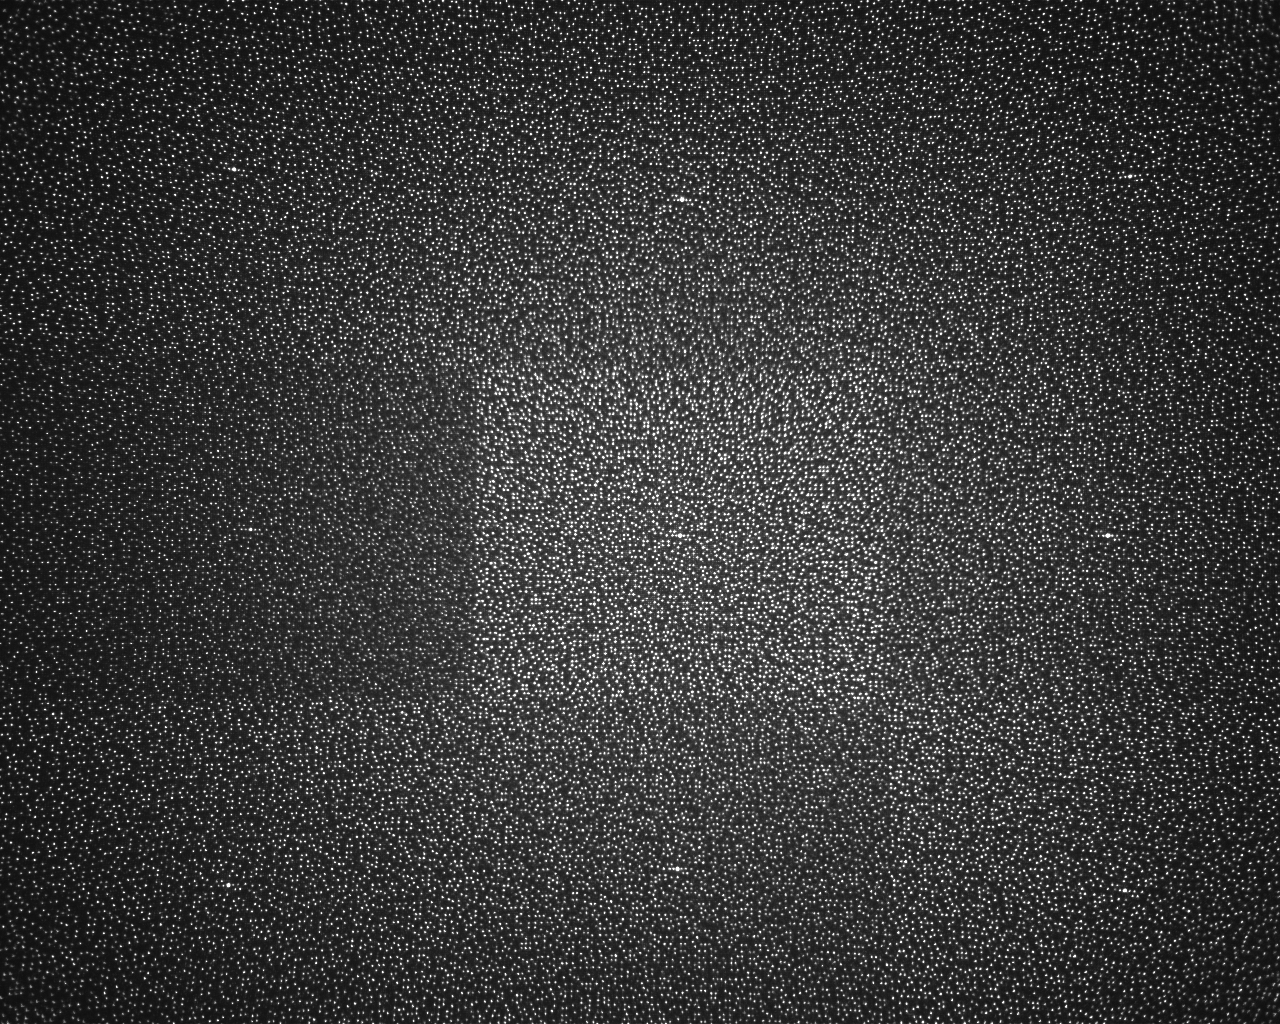
\includegraphics[width=0.9\linewidth]{figures/unproc_ref.png}
	  \caption{Nyers referencia kép}
	  \label{fig:unprocRef}
	\end{subfigure}
	\begin{subfigure}{.5\textwidth}
	  \centering
	  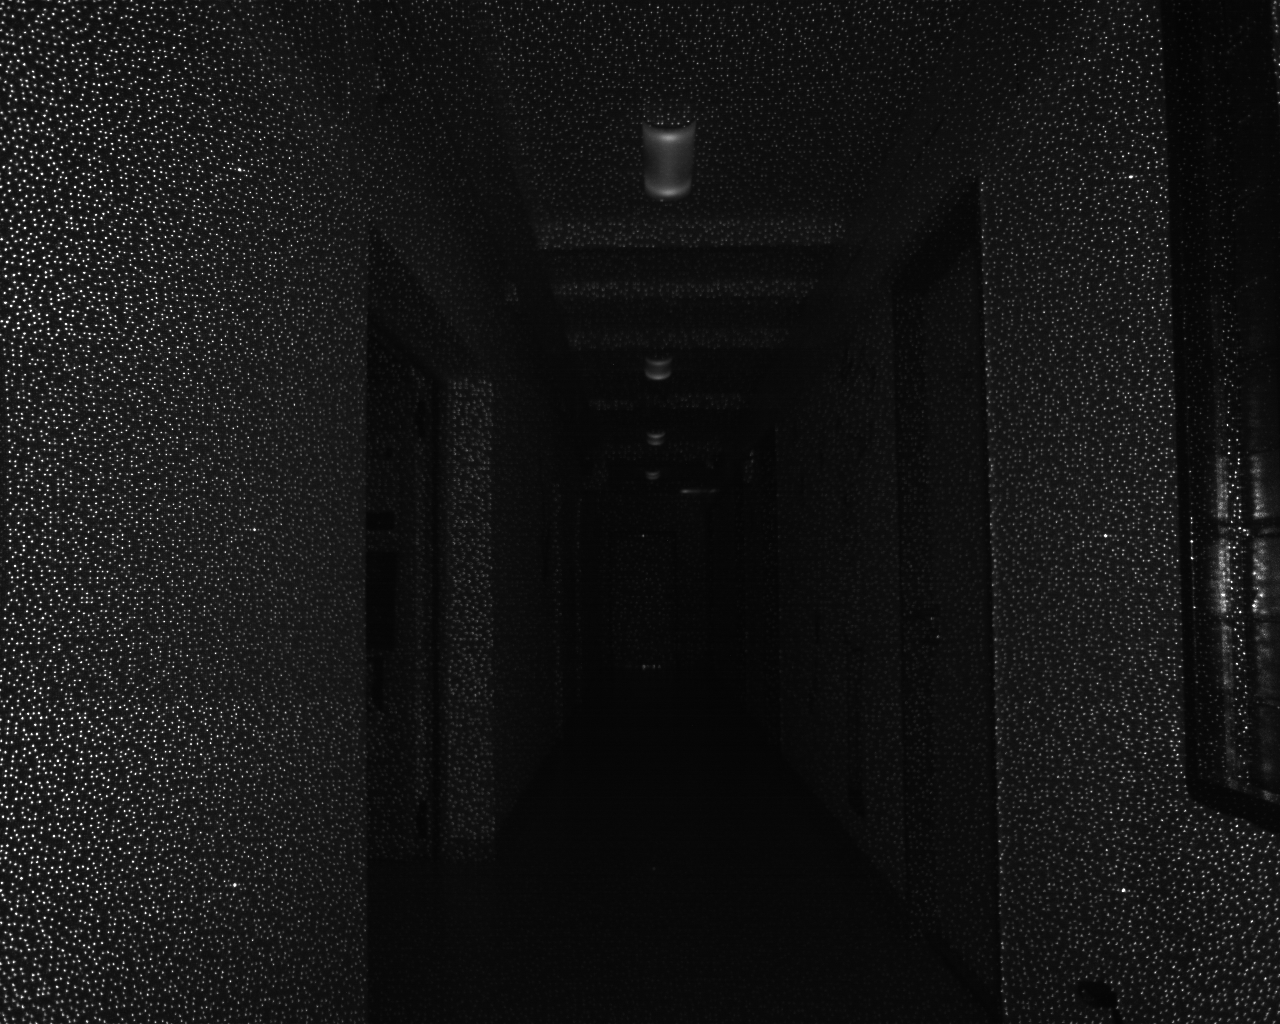
\includegraphics[width=0.9\linewidth]{figures/unproc_data.png}
	  \caption{Nyers adat kép}
	  \label{fig:unprocData}
	\end{subfigure}
	\caption{Fényviszonyok különbsége feldolgozás előtt}
	\label{fig:needToPreproc}
\end{figure}

%-----------------------------------------------------------------------------------------------
\subsection{Difference of Gaussians}\label{sect:DoG}
%-----------------------------------------------------------------------------------------------

Az első ígéretes irány a felüláteresztő szűrés volt.
Ennek egy lehetséges implementáció a DoG algoritmus.
A képet két különböző Gauss szűrővel elmossuk, majd ezeket kivonjuk egymásból.
Gyakran használt szűrő, főleg éldetektálásnál hasznos.
Az én választásom is ezért esett rá: az információ ugyan úgy megtalálható a vetített pontok kontúrjaiban, mint magukban a pontokban.
Képletszerűen \eqref{dog} írja le a műveletet. 

\begin{equation}
dst = gauss(src, \sigma_1) - gauss(src, \sigma_2)
\label{eq:dog}
\end{equation}

A szűrőnek 4 lehetséges paramétere van: a két Gauss szűrő kernel mérete valamint szórása.

%-----------------------------------------------------------------------------------------------
\subsection{Hisztogram kiegyenlítés}\label{sect:histNorm}
%-----------------------------------------------------------------------------------------------

\begin{figure}[ht!]
	\begin{subfigure}{.5\textwidth}
	  \centering
	  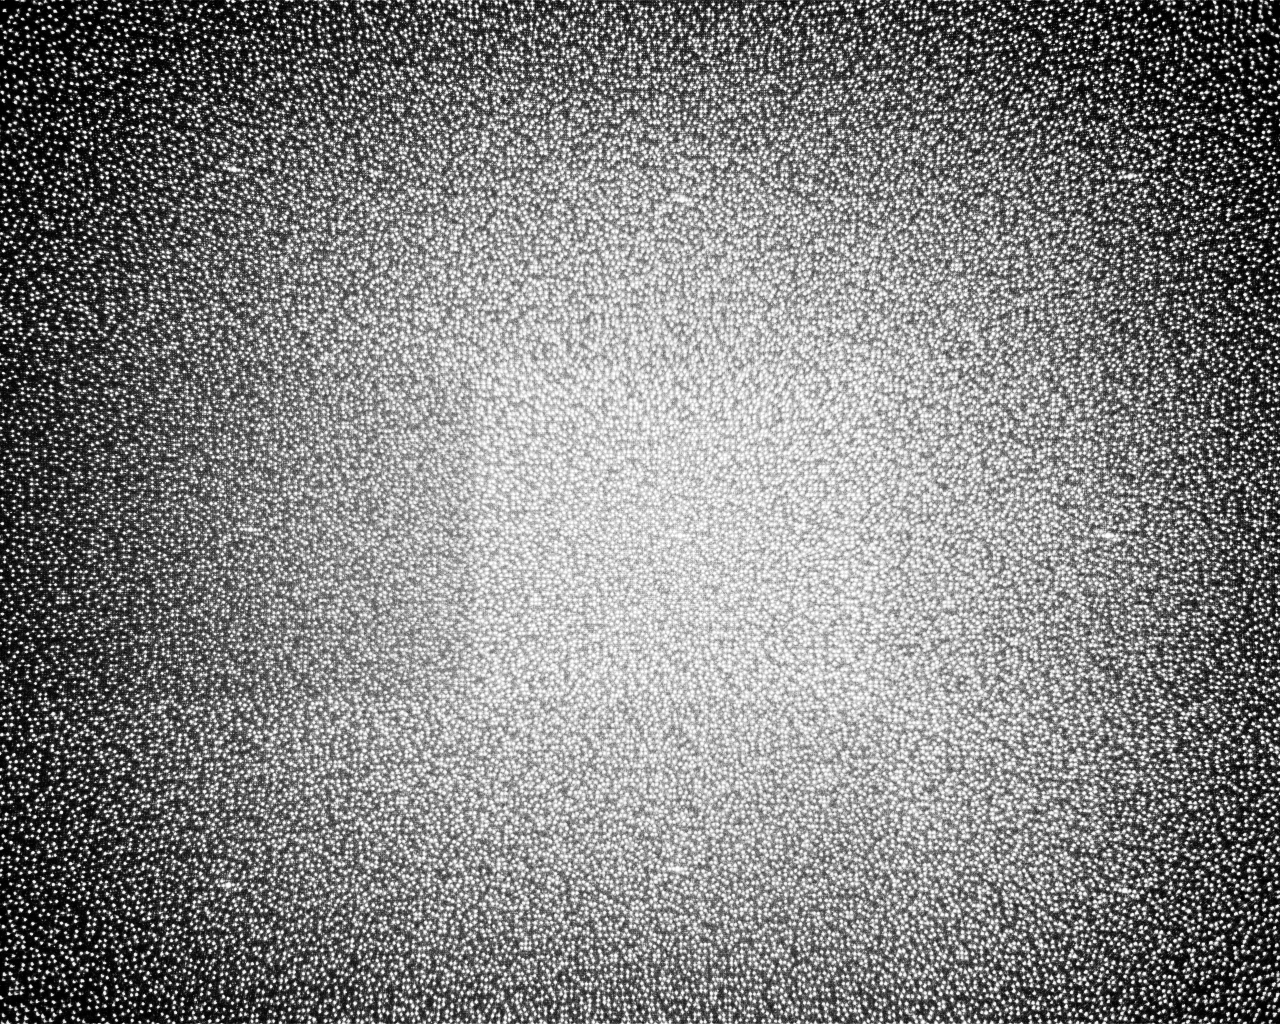
\includegraphics[width=0.9\linewidth]{figures/eq_ref.png}
	  \caption{feldolgozott referencia kép}
	  \label{fig:eqRef}
	\end{subfigure}
	\begin{subfigure}{.5\textwidth}
	  \centering
	  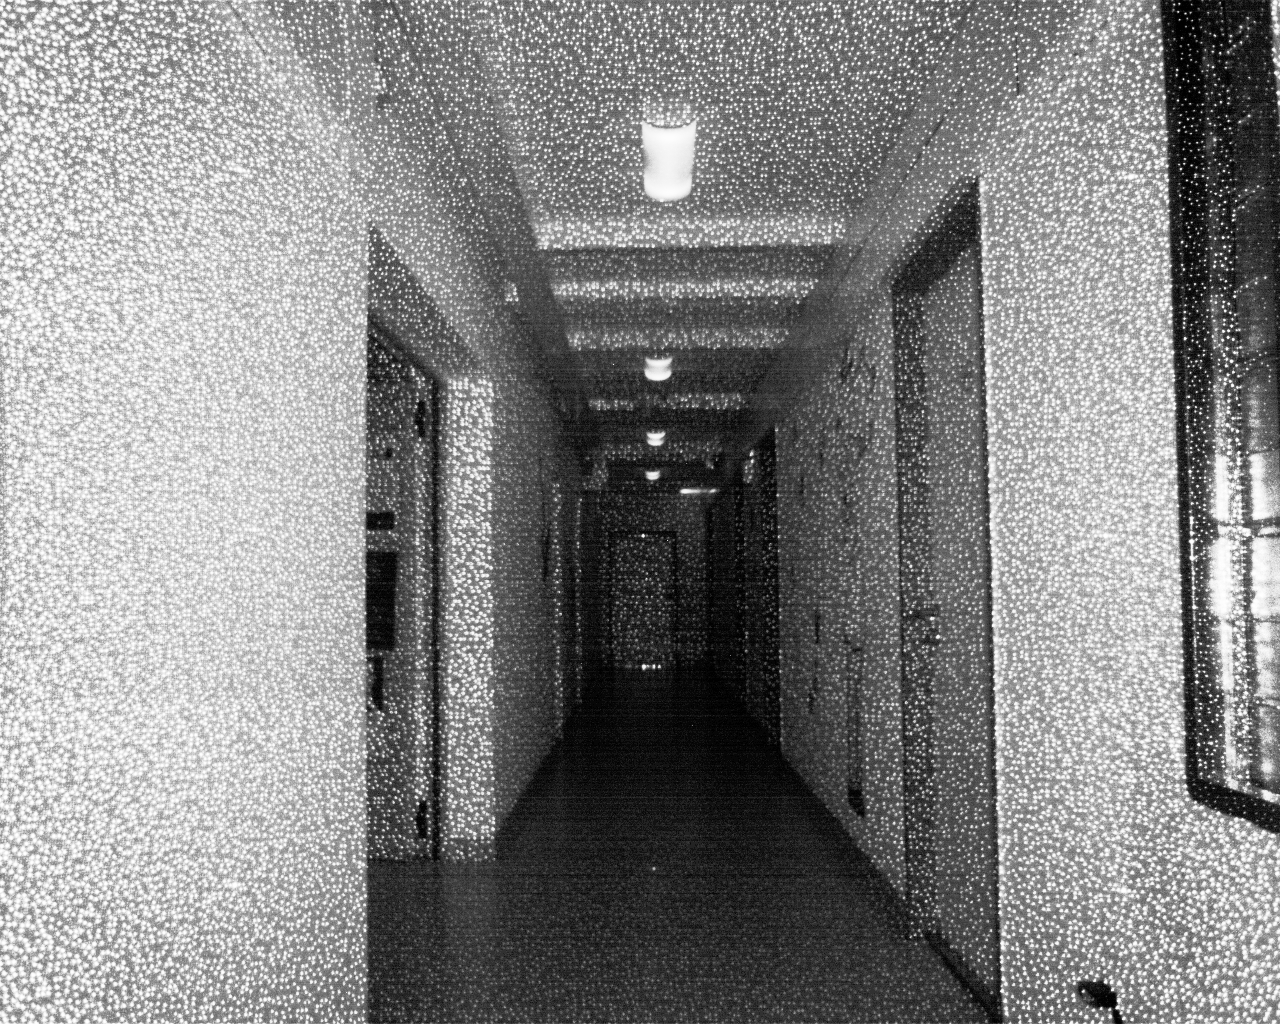
\includegraphics[width=0.9\linewidth]{figures/eq_data.png}
	  \caption{feldolgozott adat kép}
	  \label{fig:eqData}
	\end{subfigure}
	\caption{Hisztogram kiegyenlítés}
	\label{fig:eqPreproc}
\end{figure}


%-----------------------------------------------------------------------------------------------
\subsection{Egyéb előfeldolgozás}\label{sect:miscPreproc}
%-----------------------------------------------------------------------------------------------

Az itt tárgyalt eljárások lényegileg különböznek az eddigiektől.
A fenti algoritmusok a fényességkiegyenlítést szolgálják, míg az alább következők egyéb célokkal kerültek felhasználásra.

%-----------------------------------------------------------------------------------------------
\subsubsection{Uniform skálázás}\label{sect:scale}
%-----------------------------------------------------------------------------------------------

A fejlesztés során két okból került elő ez az egyszerű feldolgozási lépés.
Az első indok a futásidő csökkentése volt.
Gyorsabb volt a kisebb méretű képeken kipróbálni az egyes algoritmus változatokat, mint a teljes elérhető felbontáson.

A másik ok pedig a skálázás diszparitásképre gyakorolt hatásának vizsgálata.
Az volt a megfigyelés, hogy a felére csökkentett méretű képen (640*480) simább, kevésbé zajos a kimenet.
Ennek oka az volt, hogy azonos méretű minta nagyobb relatív méretet fedett le a képből, ezért több információt hordozott.
Ehhez adódott még hozzá az a hatás, hogy a felbontás felezése afféle aluláteresztő szűrőként viselkedik.

%-----------------------------------------------------------------------------------------------
\subsubsection{Gauss szűrés}\label{sect:gaussian}
%-----------------------------------------------------------------------------------------------

A Gauss szűrő aluláteresztő jellegű, simítja a képet.
Képfeldolgozási feladatokban gyakran alkalmazzák.
A Gauss kernel elemei egy kétdimenziós normális eloszlás mintái.
Jellemzően 3x3-as vagy 5x5-ös kernelméret a használatos (ez a kép felbontásától erősen függ).

Az két dimenziós eloszlás \eqref{gauss2d} alapján számítható.
\begin{equation}
G_0(x,y) = A e^{\frac{-(x-\mu_x)^2}{2 \sigma_x^2}+\frac{-(y-\mu_y)^2}{2 \sigma_y^2}}
\label{eq:gauss2d}
\end{equation}

A Gauss szűrő paraméterei a kernel méret és az eloszlás szórása.
Általában $\sigma_x$ és $\sigma_y$ megegyezik és négyzetes kernellel dolgozunk, de ettől természetesen el lehet térni.

%-----------------------------------------------------------------------------------------------
\section{Diszparitás meghatározás}\label{sect:Depthproc}
%-----------------------------------------------------------------------------------------------

%-----------------------------------------------------------------------------------------------
\section{Utófeldolgozás}\label{sect:Postproc}
%-----------------------------------------------------------------------------------------------


%-----------------------------------------------------------------------------------------------
\subsection{Medián szűrő}\label{sect:median}
%-----------------------------------------------------------------------------------------------


%-----------------------------------------------------------------------------------------------
\subsection{Vizualizáció}\label{sect:visual}
%-----------------------------------------------------------------------------------------------

